
\section{Allgemein}
\subsection{Spiellogik}
Unser System besteht aus zwei Komponenten. Eine Android-App mit der gesamten Spiellogik und einem Server �ber den die Kommunikation zwischen den mobilen Endger�ten abl�uft.

\subsubsection{Server}
Der implementierte Server arbeitet mit Java und ZeroMQ. Er �ffnet zwei Kommunikationskan�le mit dem Client. Der erste ist ein ZeroMQ-Request-Reply-Socket-Paar, �ber das die Endger�te Nachrichten an den Server senden. Der zweite ist ein Publish-Subscribe-Socket-Paar, �ber das die Nachrichten an Gruppen von Endger�ten weitergeleitet werden. Eine Nachricht besteht aus drei Teilen: einer Adresse, dem Nachrichtentyp und einem serialisierten Objekt vom Typ TransferObject (siehe Abbildung \ref{fig:transfer}). Die Adresse ist entweder die ID eines Spielers oder die ID einer Spielinstanz. Wir nutzen ZeroMQs Multipart-Message-Feature um diese Teile voneinander getrennt bei der Kommunikation zu �bermitteln. Der Server sendet eingehende Nachrichten an bestimmte Clients weiter. Das kann entweder ein einzelner Client, oder alle Clients die sich in einer Spielsession befinden, sein. Der Server kennt dabei den Zustand der einzelnen Spiele nicht. Um mehrere Spielinstanzen gleichzeitig verwalten zu k�nnen, h�lt er aber eine Liste aller laufenden Spiele samt Informationen dar�ber, welcher Spieler an welchem Spiel teilnimmt. Wenn eine Nachricht vom Typ "`create\_game"' empfangen wird tr�gt der Server die ID des Spiels in eine Liste ein. Diese Liste wird einem Client gesendet wenn er sie �ber eine entsprechende Nachricht anfragt.





\begin{figure}
	\begin{center}
		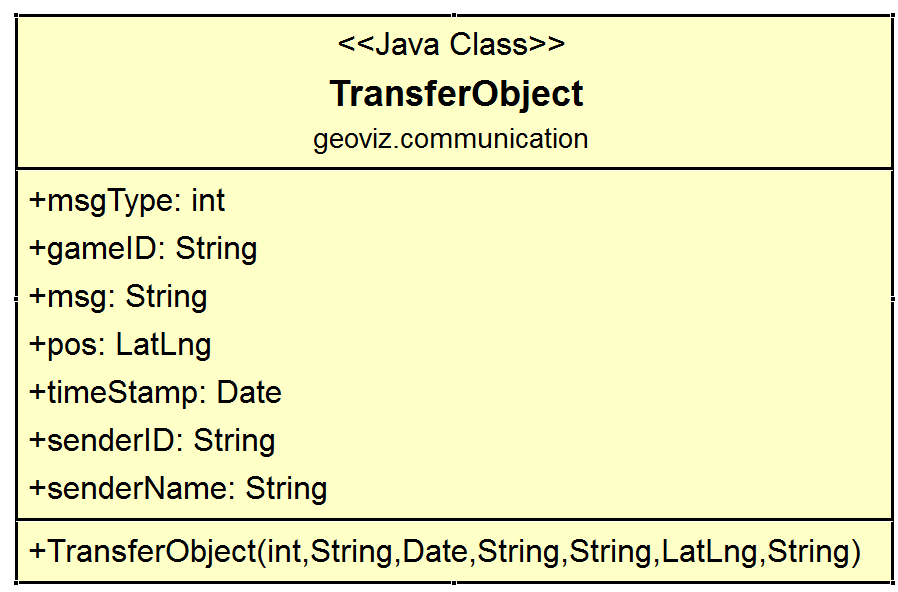
\includegraphics[width=0.5\textwidth]{img/transferobject.png}
		
		\caption{UML-Diagramm der Klasse\newline geoviz.communication.TransferObject}
		\label{fig:transfer}
	\end{center}
\end{figure}

\subsubsection{Client}
Unsere Android-Applikation besteht aus drei Fragmenten zwischen denen man durch Wischen wechseln kann. Das erste Fragment ist ein Chat �ber den Spieler Textnachrichten an ihre Mitspieler im gleichen Spiel senden k�nnen.
Das zweite Fragment ist die Karte auf der wir unser Spiel darstellen.  
F�r die Darstellung der Karte verwenden wir GoogleMaps. 
Im dritten Fragment kann ein Spieler eine neue Spielinstanz erstellen oder einem bereits laufendem Spiel beitreten. Die Liste der momentan laufenden Spiele wird per Knopfdruck vom Server abgefragt. Wenn man einer laufenden Session beitritt wird �ber den Server eine Anfrage des aktuellen Status des Spiels an alle momentanen Mitspieler gesendet, welche den Zustand des Spiels alle an den anfragenden Client zur�ck senden. Dieser beachtet nur die erste Nachricht und verwirft den Rest.
Des weiteren l�uft ein LocationClient, welcher immer die aktuelle Position als Nachricht an alle Spieler der selben Spielinstanz weiterschickt. 


 


